\cleardoublepage
\chapter{Introducción}
\label{ch:chapter1}


\section{Motivación y objetivos}\label{sec:motivación-y-objetivos}

El área del \texit{Deep Learning}~\cite{deep_learning} ha avanzado exponencialmente en los últimos años.
Esto ha permitido que a día de hoy se pueda contar con modelos predictivos capaces de procesar imágenes y clasificarlas según sus características primarias.
La consecuencia principal de este proceso es la apertura de una ventana de oportunidad a la explotación de estos modelos en un entorno real, con el objetivo de que sean cruciales a
la hora de detectar incendios, terremotos, así como todo tipo de desastres naturales.

El uso eficiente de estos modelos requiere una infraestructura capaz de soportar la fiabilidad necesaria en términos de robustez y velocidad.
En estos casos, el procesamiento en tiempo real se vuelve algo indispensable para lograr optimizar recursos de emergencia, dirigir equipos a las zonas de desastre más afectadas y, en definitiva, prevenir los máximos riesgos posibles.


Los ejes que vertebran este proyecto se sitúan en torno a dos polos: primeramente, la aceleración del tiempo de entrenamiento de un modelo de \texit{Deep Learning} usando una GPU~\cite{gpu_solution}
en el servicio de Google Colab, y en segundo lugar, la optimización del tiempo de inferencia del modelo mediante el kit de herramientas Intel OpenVINO. Finalmente, el modelo se desplegará en un entorno cloud en el que pueda funcionar como servicio capaz de soportar miles de eventos concurrentes.
Para llevar a cabo el entrenamiento del modelo se ha utilizado como herramienta principal TensorFlow~\cite{deep_learning_tensorflow}, un framework open source desarrollado por Google para la preparación de algoritmos de entrenamiento de redes neuronales.

Con la necesidad de que la aplicación sea robusta y flexible ante cambios se ha usado la tecnología de contendores Docker\footnote{\rule{https://www.docker.com/}}.
Empleando esta herramienta se asegura que tanto las versiones del sistema operativo como de librerías externas sean compatibles entre sí, adicionalmente, se deja abierta la posibilidad de portar la aplicación a distintos entornos que aprovechen esta solución de contenedores.
La consecución del objetivo general anteriormente mencionado se lleva a cabo en la presente memoria abordando una serie de objetivos específicos, los cuales se enumeran a
continuación:
\begin{itemize}
    \item Mejora en los tiempos de entrenamiento de un modelo de
    \texit{Deep Learning} usando una GPU del servicio de Google Colab.
    \item Conversión de un modelo de TensorFlow a uno de OpenVINO para aumentar su velocidad de inferencia.
    \item Preparación de una arquitectura de Google cloud capaz de soportar tráfico concurrente en tiempos óptimos para el servicio.
    \item Codificación de una aplicación capaz de hacer uso de los distintos sistemas de inferencia de TensorFlow y OpenVINO\@.
    \item Codificación de una aplicación web apta para exponer todos los servicios en un entorno productivo.
    \item Encapsulación de los distintos entornos de producción haciendo uso de Docker.
    \item Despliegue de la aplicación y pruebas de carga.
    \item Obtención de resultados y realización de comparativas de rendimiento entre los distintos sistemas de inferencia, hardware y servidores web.
\end{itemize}


\section{Estado del arte}\label{sec:estado-del-arte}
En la actualidad, la inteligencia artificial se compone de varias ramas tales como machine learning, natural language processing, entre otras. Una de ellas es el \texit{Deep Learning}.
Esta arquitectura de aprendizaje profundo persigue el estudio y clasificación de una variedad de problemas
haciendo uso de sus propios algoritmos.
Actualmente, los algoritmos de \texit{Deep Learning} son usados para todo tipo de problemas que abarcan multitud de sectores dentro de la industria \cite{robotics}, los gobiernos y en definitiva, de la propia sociedad. La digitalización y expansión de internet provee de innumerables fuentes de datos capaces de ser procesadas y analizadas por este tipo de algoritmos, que son usadas para distintos fines.

El propio origen de los datos ha cambiado, ahora provienen de interacciones que tienen los usuarios con sus dispositivos móviles, llamadas, transacciones de dinero por internet \cite{crypto}, navegación de páginas web y, en el caso de este trabajo, imágenes de un satélite.
El tratamiento de imágenes ha supuesto un avance en la sociedad del que ahora se aprovechan cuerpos de policía, usando estas herramientas para detección de matrículas o el reconocimiento de potenciales delincuentes\footnote{\url{https://www.nhtsa.gov/sites/nhtsa.dot.gov/files/documents/809811-lidarspeedmeasuringdevice.pdf}}; médicos, que utilizan estos sistemas \cite{medic} para mejorar la detección prematura de algunos tipos de cáncer\footnote{\url{https://www.nature.com/articles/srep46450}}, o en el caso de la industria, que se ayuda de estas soluciones para automatizar y clasificar procesos que antes suponían la supervisión o ejecución de una persona.
Del mismo modo, los países poseen sus sistemas personales de reconocimiento de imágenes para la clasificación de sus ciudadanos, sistemas de recomendación tanto para las empresas que buscan aumentar sus ventas como para bancos que buscan personas aptas para préstamos e incluso sirve como sesgo para evitar contenido indeseable en plataformas a través de la red.


En general, la cantidad masiva de datos ha creado una necesidad de explotación a
través de los mismos, por lo que el \texit{Deep Learning} se sitúa como una herramienta fiable para dar valor a todas las interacciones que están ocurriendo casi de manera permanente
en cada sistema tecnológico del planeta.
Todo este estímulo lleva consigo la creación de miles de nuevos puestos de trabajo en el sector tecnológico, dedicados en exclusiva a la aplicación de algoritmos de aprendizaje automático, de igual manera que al aumento de su enseñanza.
Esto ha abierto la posibilidad a profesionales que anteriormente no tenían una función claramente definida en este campo a situarse como prácticamente indispensables.
Los beneficios son perceptibles en estudios como matemáticas, estadística y relacionados. En estos ámbitos, el perfil matemático y la capacidad de análisis son aptitudes muy valoradas para la realización de este tipo de tareas.

El desarrollo de este nuevo perfil de profesionales ha fomentado el empleo de lenguajes de programación menos usuales hasta el momento. Esto se debe a que tanto su uso como curva de aprendizaje es más asequible que el de otros lenguajes más tradicionales, caso de Java o C++ (ver Figura~\ref{fig:Encuesta_sobre_lenguajes_de_programación_en_StackOverflow_2019}). Junto a ello, han surgido nuevas herramientas  gratuitas y de código abierto \cite{open}, tales como Jupyter, TensorFlow, Scikit-learn o PyTorch, entre otras.


\begin{figure}
    \centering
    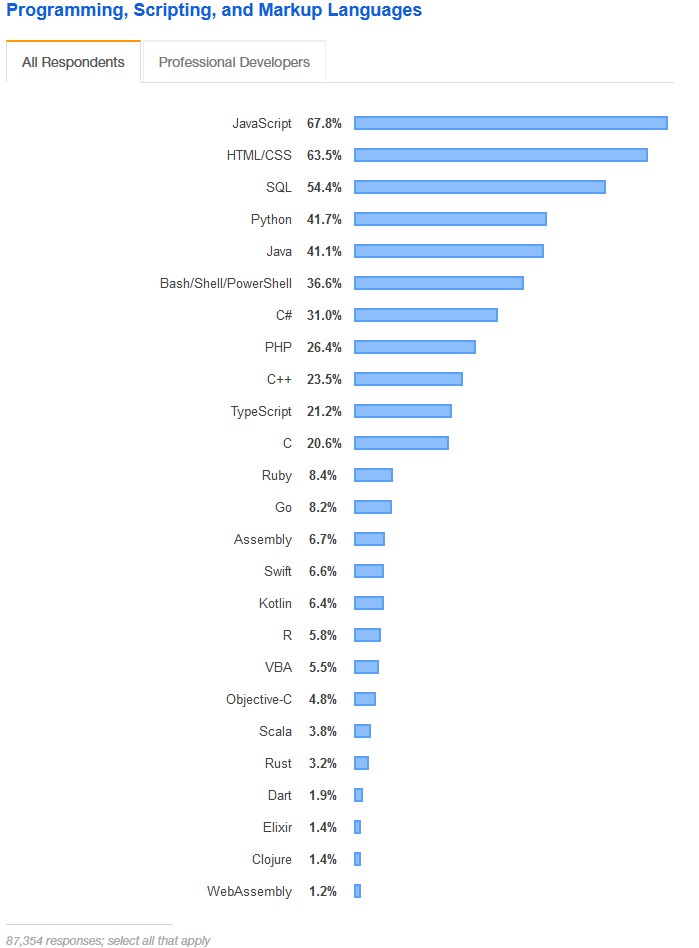
\includegraphics[width=0.95\textwidth]{images/chapter1/stackoverflow_language.png}
    \caption{Encuesta sobre lenguajes de programación usados en StackOverflow 2019.}
    \label{fig:Encuesta_sobre_lenguajes_de_programación_en_StackOverflow_2019}
\end{figure}

\subsection{Concepto Deep Learning}\label{subsec:concepto-deep-learning}

El \texit{Deep Learning} tiene como elemento definitorio el uso de algoritmos que basan su estructura en redes neuronales artificiales, imitando el comportamiento que tienen las del ser humano y su sistema nervioso central.
La fuerza que ha proporcionado el surgimiento del Big Data ha conseguido que este tipo tecnologías se conviertan en la práctica diaria de muchos profesionales.
Una de las claves de los algoritmos de \texit{Deep Learning} está en la capacidad de aprendizaje que reside en ellos.
Esto nos brinda la posibilidad de lidiar con problemas del mundo real,
en el que las combinaciones de posibilidades y reconocimiento de patrones se quedan fuera de nuestros cálculos.
Las redes neuronales representan la principal herramienta para clasificar imágenes. Esto es debido a que pueden extraer características fundamentales de cada píxel y poseen un alto porcentaje de acierto en la predicción.


Para poder materializar todos estos algoritmos de aprendizaje automático disponemos de servicios de grandes empresas como Google, Amazon e IBM, que
implementan sus propias soluciones comerciales \cite{cloudComputing}.
Pero también podemos optar por herramientas de código abierto como TensorFlow, una de las librerías más famosas de \texit{Deep Learning} desarrollada por los ingenieros de Google, posteriormente liberada bajo licencia Apache.
También disponemos de otras como PyTorch y Keras.
Todas las mencionadas anteriormente fueron originalmente desarrolladas para el lenguaje de programación Python, el cual ha visto aumentado su porcentaje de uso debido a esta corriente de
machine learning \cite{python_machine}.

\subsection{Redes neuronales en el tratamiento de imágenes}\label{subsec:redes-neuronales-en-el-tratamiento-de-imágenes}
La unidad básica de procesamiento de las redes neuronales es el perceptrón (ver Figura~\ref{fig:Perceptrón_}),
a partir del que se desarrolla un algoritmo capaz de generar criterios de selección de subconjuntos de neuronas.
Este conjunto de neuronas pasará a formar parte de las distintas capas que componen por completo la red neuronal.
Cada neurona recibe una entrada, ya sea de una fuente externa o de otra neurona.

\begin{figure}[H]
    \centering
    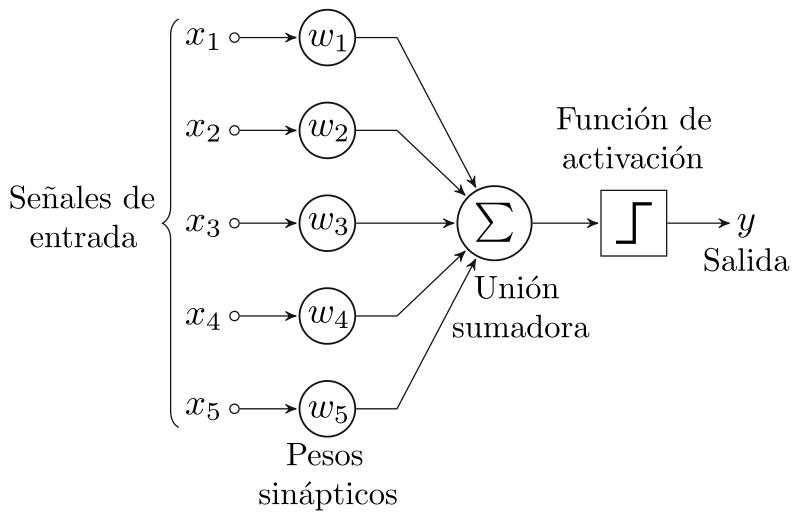
\includegraphics[width=0.6\textwidth]{images/chapter1/perceptron.png}
    \caption{Ejemplo de perceptrón.}
    \label{fig:Perceptrón_}
\end{figure}

Cada neurona aplica una función de cálculo a partir de la cual se generan los pesos correspondientes de cada neurona. Estos pesos representan el nivel de interacción de las neuronas y deberán de ser ajustados de manera que se ciñan lo más posible a los datos que conocemos.
Los pesos de entrada de una capa tienen origen en una capa anterior y sus salidas forman parte de la entrada de una capa posterior. La propagación se produce hasta llegar a la última capa de la red, que será la capa de salida de la que obtengamos el resultado de nuestra clasificación.

En este problema concreto nos centramos en clasificar imágenes multiespectrales con alta resolución espacial \cite{imageProcessing} haciendo uso de las bandas espectrales RGB (Red, Green and Blue).
Nuestro conjunto de imágenes pertenece a una zona parcialmente destruida por un desastre natural en Haití, ocurrido en el año 2010.
Estas imágenes fueron adquiridas por el satélite de observación terrestre de alta resolución GeoEye-1, lanzado en septiembre de 2008.
Por lo tanto, el fin de nuestro modelo de \texit{Deep Learning} es tener la capacidad de clasificar dichas imágenes dependiendo si la zona está dañada o, por el contrario, está en buenas condiciones.

\section{Plan de trabajo}\label{sec:plan-de-trabajo}
En la Figura~\ref{fig:Plan_de_trabajo} podemos observar el plan de consecución de objetivos seguidos en este trabajo.
La métrica de esfuerzo que aparece en ella hace referencia al número de jornadas invertidas en cada tarea, con una suma total de 10 semanas.
Las actividades están ordenadas de manera secuencial en su ejecución y presentan una dependencia entre sí, por lo que nunca se ha
pasado a otra tarea sin completar la anterior.

\begin{figure}[H]
    \centering
    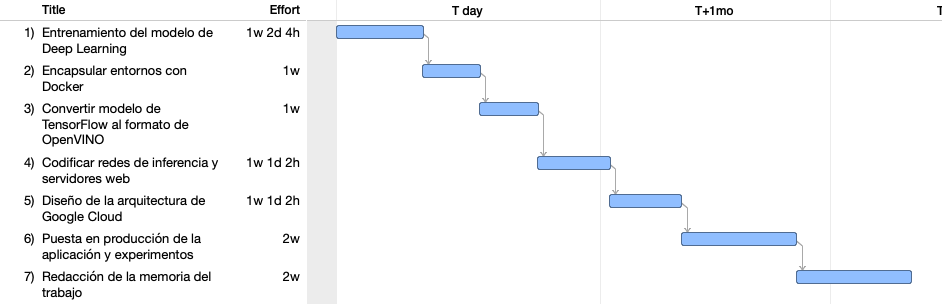
\includegraphics[width=1\textwidth]{images/chapter1/work_plan.png}
    \caption{Plan de trabajo.}
    \label{fig:Plan_de_trabajo}
\end{figure}

\section{Organización de esta memoria}\label{sec:organización-de-esta-memoria}

Teniendo presentes los anteriores objetivos concretos, se procede a describir la organización del resto de esta memoria, estructurada en una serie de capítulos cuyos contenidos se
describen a continuación:

\begin{itemize}
    \item \textbf{Entrenamiento del modelo mediante Google Colab}: Se define el proceso de entrenamiento y aumento de la velocidad usando la plataforma Google Colab y su hardware asociado.
    \item \textbf{Tecnología OpenVINO}: Se define el propósito del kit de herramientas de Intel OpenVINO así como la transformación de un modelo de TensorFlow para que sea compatible con dicha solución.
    \item \textbf{Arquitectura Cloud propuesta}: Se presenta la arquitectura de Google Cloud diseñada para soportar toda la infraestructura de la aplicación y se explica la puesta en producción del servicio.
    \item \textbf{Resultados experimentales}: Se preparan los distintos frameworks web que van a ser puestos a prueba haciendo uso del lenguaje de programación Python, mostrando el rendimiento obtenido en las fases de entrenamiento y de inferencias. Además, se presentará el cálculo aproximado de los costes del proyecto.
    \item \textbf{Conclusiones y trabajo futuro}: Se presentan las conclusiones obtenidas mediante las pruebas de carga y también algunas posibles líneas de trabajo futuro que se pueden desempeñar en relación al presente trabajo.
\end{itemize}